\documentclass[11pt,xcolor=svgnames]{beamer}
\usepackage{dsfont,natbib,setspace,changepage,multirow,textcomp}
\mode<presentation>

% replaces beamer foot with simple page number
\setbeamertemplate{navigation symbols}{}
\setbeamercolor{frametitle}{fg=black}
\setbeamerfont{frametitle}{series=\bfseries}
\setbeamerfont{frametitle}{size=\normalsize}
\newcommand{\theme}{\color{Maroon}}

\setbeamertemplate{footline}{
   \raisebox{5pt}{\makebox[\paperwidth]{\hfill\makebox[20pt]{\color{gray}\scriptsize\insertframenumber}}}}

\usepackage{tikz}

\graphicspath{{../graphs/}}

\setbeamercolor{whitebox}{bg=gray!10}

% colors
\newcommand{\bk}{\color{black}}
\newcommand{\rd}{\color{red}}
\newcommand{\fg}{\color{ForestGreen}}
\newcommand{\bl}{\color{blue}}
\newcommand{\gr}{\color{black!60}}
\newcommand{\sg}{\color{DarkSlateGray}}
\newcommand{\br}{\color{SaddleBrown}}
\newcommand{\nv}{\color{Navy}}


% common math markups
\newcommand{\bs}[1]{\boldsymbol{#1}}
\newcommand{\mc}[1]{\mathcal{#1}}
\newcommand{\mr}[1]{\mathrm{#1}}
\newcommand{\bm}[1]{\mathbf{#1}}
\newcommand{\ds}[1]{\mathds{#1}}
\newcommand{\indep}{\perp\!\!\!\perp}

% spacing and style shorthand
\setstretch{1.1}

% shorthand
\newcommand{\sk}{\vspace{.5cm}}
\newcommand{\R}[1]{{\tt \nv #1}}
\newcommand{\til}{{\footnotesize$\bs{\stackrel{\sim}{}}$}}
\DeclareSymbolFont{extraup}{U}{zavm}{m}{n}
\DeclareMathSymbol{\vardiamond}{\mathalpha}{extraup}{87}

\begin{document}

\setcounter{page}{0}
{ \usebackgroundtemplate{
\includegraphics[height=\paperheight]{phoenix}}
\begin{frame}[plain]
\begin{center}


{\bf \Large [5] Big Data: Classification}

\vskip 1.5cm 
Matt Taddy, University of Chicago Booth School of Business

\vskip .2cm 
\texttt{faculty.chicagobooth.edu/matt.taddy/teaching} 


\end{center}
\end{frame} }


\begin{frame}
{[5] \theme Classification }

\sk
$K$-nearest neighbors and group membership.

\sk
Binary classification: { from probabilities to decisions.}
\begin{itemize}
\item Misclassification, sensitivity and specificity.
\end{itemize}

\sk 
Multinomial logistic regression: fit and probabilities.

\sk
DMR and {\nv distributed computing}.


\end{frame}

\begin{frame}
{Nearest Neighbors}


In classification, $y$ is membership in a category
$\left\{ { 1}, { 2}, ..., { m}\right\}$.

\vskip .1cm
Each class observation $y_i$ is accompanied by covariates
  $\bm{x}_i$.

\vskip .1cm
{The classification problem:} given new $\bm{x}$ what is
  $\hat{y}$? 

\sk
{\bf {\nv  KNN:} what is the most common class around x?}

\vskip .1cm
Take your $K$-nearest neighbors
$\bm{x}_{i_1}\ldots\bm{x}_{i_k}$, and let them vote.

\vskip .1cm
Nearness is in euclidean distance:
$\sqrt{\sum_{j=1}^p(x_j-x_{ij})^2}$. {\gr (units!)}

\vskip .1cm
$\hat{y}$ is assigned the most common category in $\{y_{i_1}\ldots y_{i_k}\}$.

\sk
Since we're calculating distances on $\bm{X}$, scale Matters!\\

\bk We'll use R's scale function to divide each $x_j$ by $\mr{sd}(x_j)$ 

\gr The new units of distance are in {\it standard deviations}. 
\end{frame}


\begin{frame}
{Nearest Neighbors}

\begin{columns}[c] 
\column{2in}
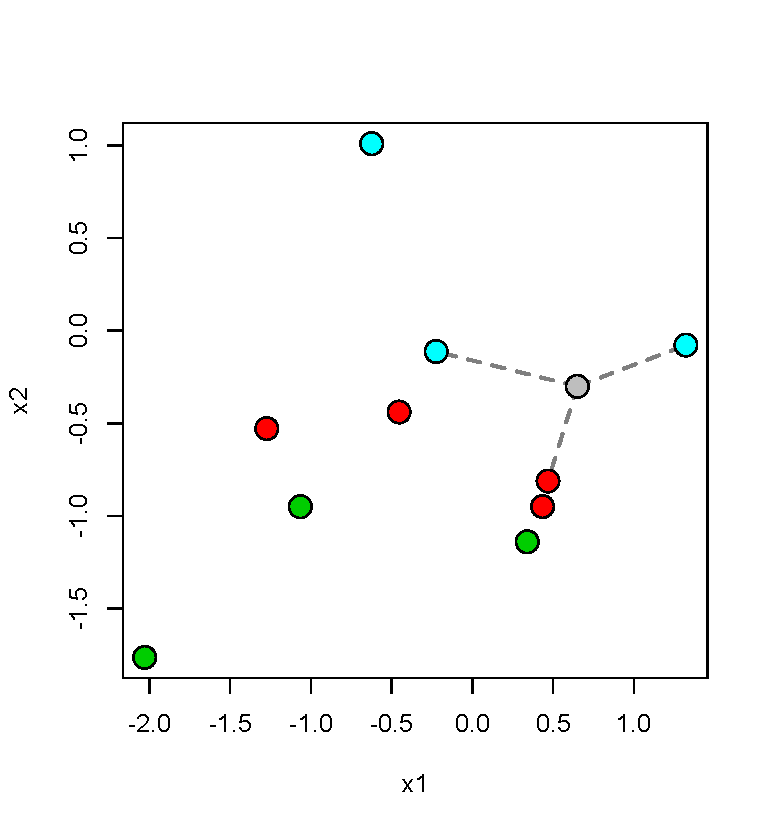
\includegraphics[width=2in]{../graphs/nearest}
\column{2.5in}
$K$-NN's collaborative estimation:

\vskip .1cm
\hfill   Each neighbor votes.~~~~~~~

\sk
Neighborhood is by shortest distance (shown as the dashed lines).

\sk The relative vote counts provide a {\theme very crude} estimate of probability.
\end{columns}

\bk\vskip .25cm
For 3-nn, $\nv\mr{p}(\text{blue}) = 2/3$,  but for 4-nn or 2-nn, it's
only {\nv 1/2}.\\\gr
Sensitive to neighborhood size (think about extremes: {\it
  1}  or $n$).


\end{frame}


\begin{frame}
{Forensic Glass Analysis}

\sk
\begin{columns}

\column{2.6in}

~~~~~~~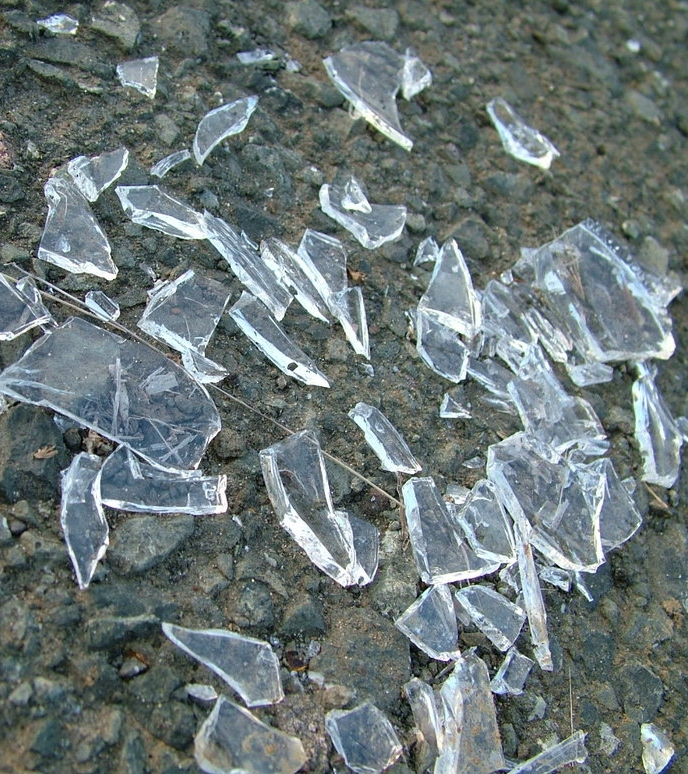
\includegraphics[width=2in]{../graphs/FGLbroken}

\column{2.5in}

{\nv Classifying shards of glass}\\
Refractive index, plus oxide \%\\
{Na, Mg, Al, Si,
K, Ca, Ba, Fe.}

\vskip .3cm
~~{\nv 6 possible glass types}\\
~~{\bk \tt WinF:} float glass window\\
~~{\bk \tt WinNF:} non-float window\\
~~{\bk \tt Veh:} vehicle window\\
~~{\bk \tt Con:} container (bottles)\\
~~{\bk \tt Tabl:} tableware\\
~~{\bk \tt Head:} vehicle headlamp\\

\end{columns}
\end{frame}


\begin{frame}
{Glass Data: characteristic by type}

\sk
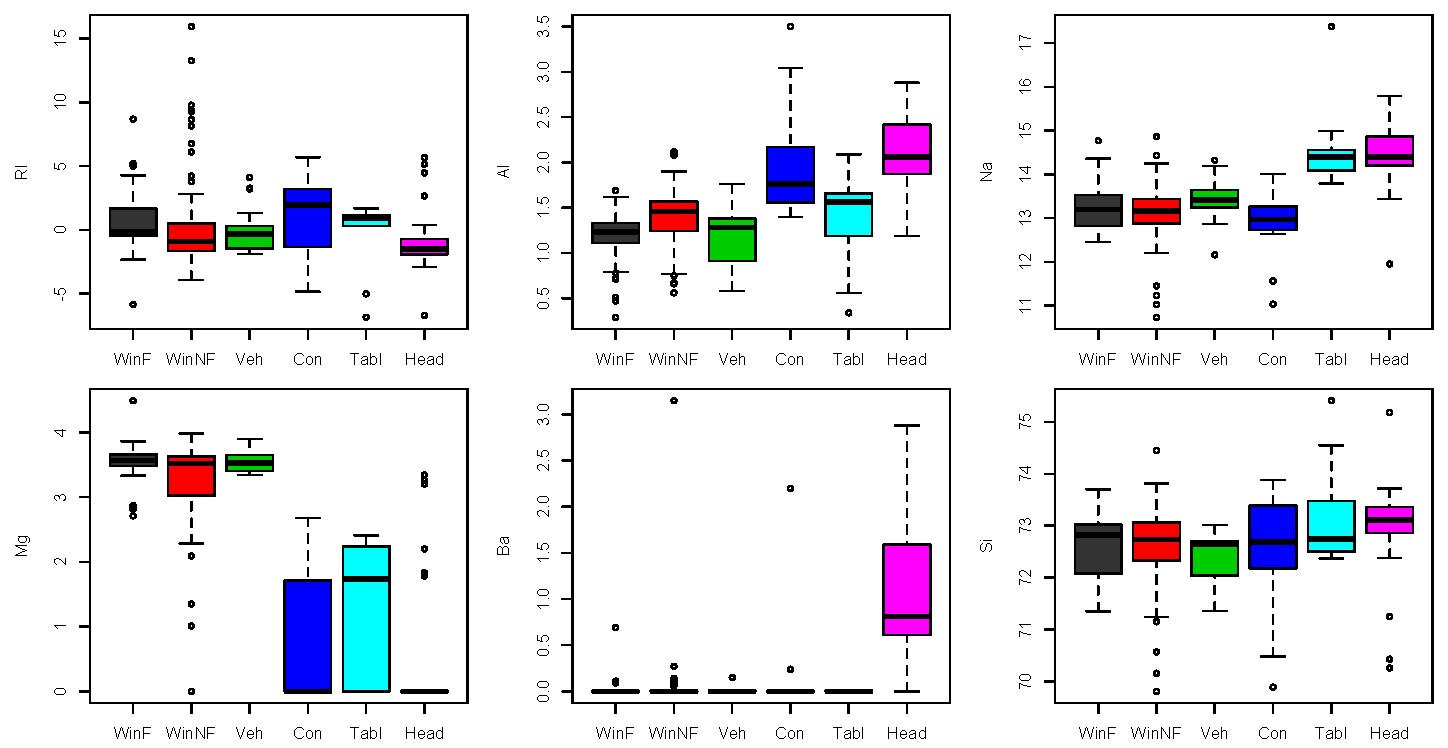
\includegraphics[width=4.25in]{FGLdata}

\sk
Some covariates are clear {\theme discriminators} {\gr (Ba for
  headlamps, Mg for windows)} while others are more subtle
{\gr(Refractive Ind)}.

\end{frame}


\begin{frame}[fragile]
{Nearest neighbors in R}

\vskip .25cm
{Load the \R{class} package  which includes function
\R{knn}.}

\vskip .1cm
\R{train} and \R{test} are covariate matrices,
\R{cl} holds known $y$'s.

\vskip .1cm

You set \R{k} to specify how many neighbors get to vote.

\vskip .1cm

Specify \R{prob=TRUE} to get neighbor vote proportions.

\begin{semiverbatim}\nv\footnotesize
knn(train=xobserved, test=xnew, cl=y, k=3) 
nn1 <- knn(train=x[ti,], test=x[-ti,], cl=y[ti], k=1)
nn5 <- knn(train=x[ti,], test=x[-ti,], cl=y[ti], k=5)
data.frame(ynew,nn1,nn5)\bk
          ynew      nn1      nn5
          WinF     WinF     WinF
           Con      Con     Head
          Tabl    WinNF    WinNF
\end{semiverbatim}

\end{frame}


\begin{frame}
{KNN classification in the RI$\times$Mg plane.}

\begin{adjustwidth}{-.1in}{}\vskip -.5cm
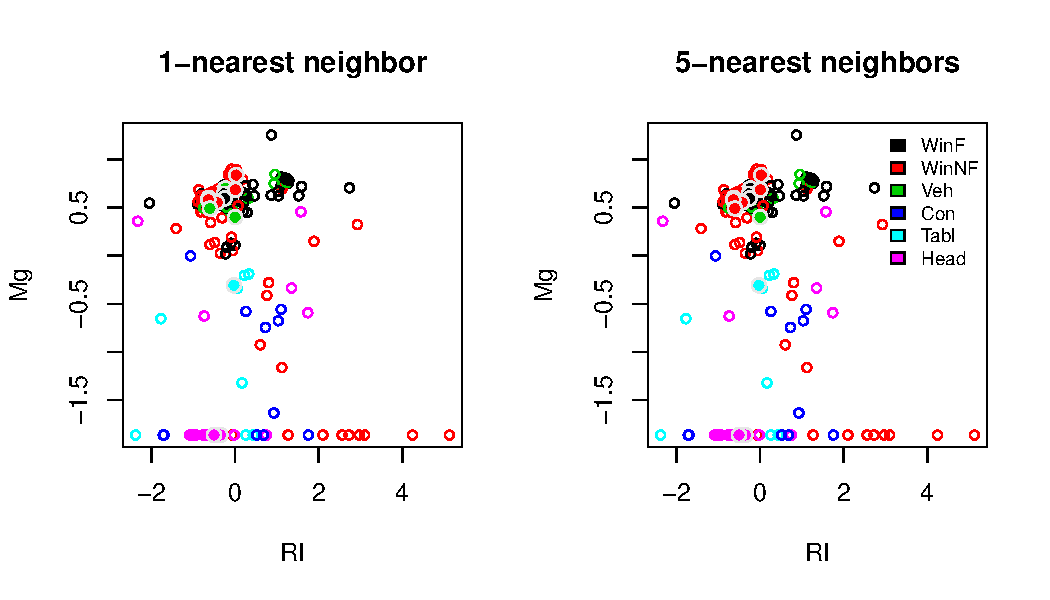
\includegraphics[width=4.5in]{FGLknn}
\end{adjustwidth}

{\gr Open circles are observations and closed are predictions.}

\vskip .1cm
\hfill The number of neighbors matters!~~~~~~~~

\vskip -.25cm
\end{frame}


\begin{frame}
{Limits of KNN}

{Nearest neighbors is  simple, but limited}

\sk
There is no good way to choose $K$.

\vskip .1cm
Cross-validation works, but is unstable: new data $\Rightarrow$
new $K$.

\vskip .1cm
{And the classification is {\it very} sensitive to $K$}.

\sk 
All you get is a classification, with only rough 
probabilities.

\vskip .1cm
These are often zero or one: useless in making decisions.

\vskip .1cm
{\nv Without probabilities, you cannot  assess
misclassification risk.}

\sk
But the basic idea is the same as in logistic regression:
\\
~~Observations with similar $\bm{x}$'s should be classified similarly.

\end{frame}

\begin{frame}
{Probability, cost, and classification}


Many decisions can be reduced to binary classification.

\vskip .2cm
There are two ways to be wrong in a binary  problem.

\vskip .25cm
~~~~~ False {\fg positive}: {predict $\hat{y}=1$ when $y=0$.}\\
~~~~~ False {\rd negative}: {predict $\hat{y}=0$ when $y=1$.}

\vskip .25cm
There will be  costs associated
with each type of error.

\sk
{To make optimal decisions, you need to estimate
  probabilities.}

\vskip .1cm
Once you know $\hat{p}$, the probability of $y=1$, you can assess
risk.


\vskip .1cm
We know how to estimate probabilities: logistic regression!


\end{frame}


\begin{frame}

\begin{adjustwidth}{-.4in}{}
\vskip -.5in

\includegraphics[width=5.1in]{../graphs/CREDcards}
\end{adjustwidth}

\vskip .25cm
{\Large Credit Classification}

\sk
Credit scoring is a classic problem of classification.

\vskip .2cm
Take borrower/loan characteristics and 
previous defaults,\\ use these to predict performance of potential new loans.
{\gr
Bond-rating is a multi-class extension of the problem.}

\vskip .25cm 
Consider the German loan/default data in {\tt credit.csv}.
\begin{itemize}
\item Borrower and loan characteristics: {\gr job, installments, etc.}
\item Pretty messy data, needs a bit of a clean...  
\end{itemize}

\end{frame}


\begin{frame}
{Choice Sampling}

{A caution on retrospective sampling}

\begin{adjustwidth}{-.2in}{} \vskip -.75cm
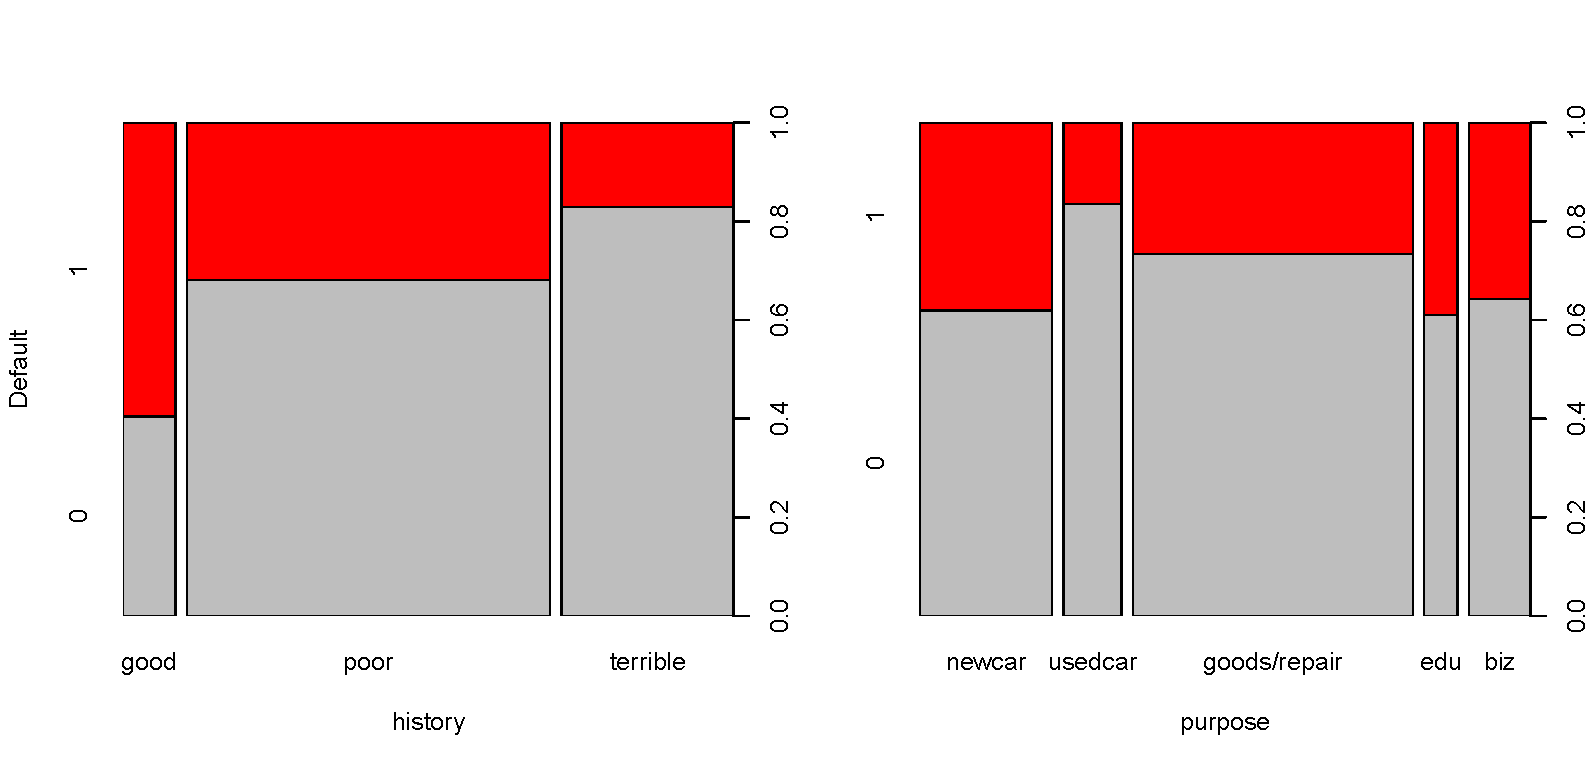
\includegraphics[width=4.5in]{../graphs/CREDmosaic}
\end{adjustwidth}


See anything strange here?  Think
about your data sources! 

\vskip .1cm Conditioning helps here, but won't always solve everything...

\end{frame}

\begin{frame}[fragile]
{German Credit Lasso}

\vskip .25cm
{
Create a numeric $\bm{x}$ and run lasso logistic regression.}

\vskip .25cm
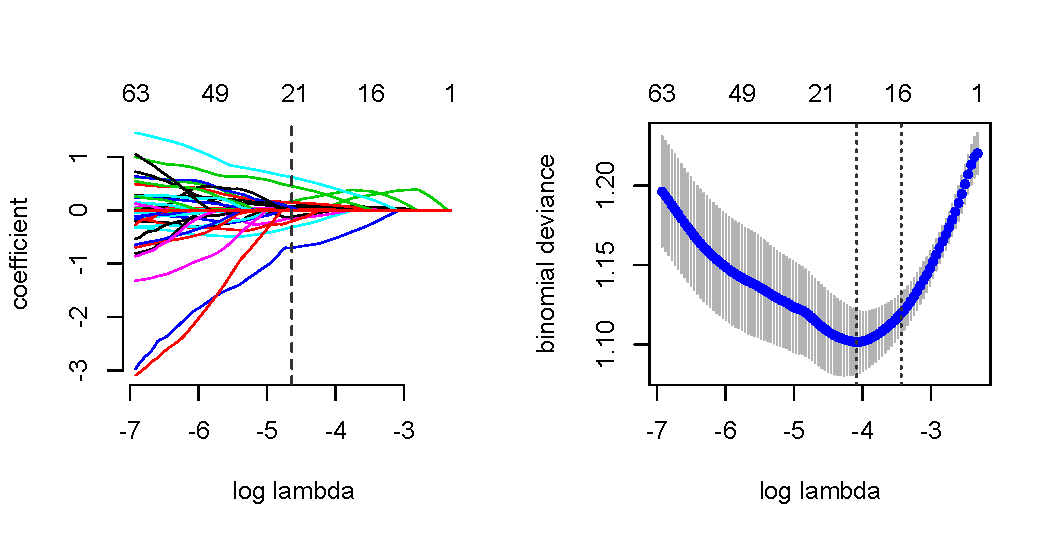
\includegraphics[width=4.25in]{CREDlasso}

\begin{semiverbatim}\small\nv
> sum(coef(credscore)!=0){\theme 13}{\gr # cv.1se}
> sum(coef(credscore, s="min")!=0){\theme 21}{\gr # cv.min}
> sum(coef(credscore\$gamlr)!=0){\theme 21}{\gr # AICc}
\end{semiverbatim}

\end{frame}



\begin{frame}
{Using probabilities to make decisions}

\vskip .25cm
Say that, on average, for every 1\$ loaned you make \\25\textcent~in interest if it is repayed but lose 1\$ if they default.

\vskip .1cm
This gives the following action-{\it cost} matrix
\begin{center}
\begin{tabular}{r|cc}
&{\it payer} & {\it defaulter}\\
\cline{2-3}
{\it loan} & -0.25 & 1\\
{\it no loan} & 0 & 0\\
\end{tabular}
\end{center}


Suppose you estimate $p$ for the probability of default.\\
Expected {\it profit} from lending is greater than zero if
\[
(1-p)\frac{1}{4} - p > 0 ~~\Leftrightarrow~~ \frac{1}{4} > \frac{5}{4}p
~~\Leftrightarrow~~  \theme p < 1/5
\]
So, from this simple matrix you should lend\\ whenever probability of default is less than 0.2.

\end{frame}


\begin{frame}[fragile]
{FP and FN Rates}

{Any classification cutoff (e.g., our $p=1/5$ rule, built from an expected profit/loss analysis) has some basic properties.}

\vskip .25cm
{\theme False Positive Rate:} \# misclassified as pos / \# classified pos.

\vskip .1cm
{\theme False Negative Rate:} \# misclassified as neg / \# classified neg.


\vskip .25cm

In-Sample rates for our $p=1/5$ rule:
\begin{semiverbatim}\small\nv
{\gr## false positive rate}
> sum( (pred>rule)[default==0] )/sum(pred>rule) 
\bk[1] 0.6704289\nv
{\gr## false negative rate}
> sum( (pred<rule)[default==1] )/sum(pred<rule)\nv
\bk[1] 0.07017544
\end{semiverbatim}
For comparison, a $p=\frac{1}{2}$ cut-off gives FPR=0.27, FNR=0.28.
\end{frame}

\begin{frame}[fragile]
{Sensitivity and Specificity}

{Two more common classification rates are}

 ~~{\it sensitivity}: proportion of true $y=1$ classified as such.\\
 ~~{\it specificity}: proportion of true $y=0$ classified as such.

\vskip .2cm
A rule is 
{\nv sensitive} if it predicts $1$ for
most $y=1$ observations, and 
{\nv specific} if it predicts $0$ for most $y=0$ observations.
\begin{semiverbatim}\small\nv
> mean( (pred>1/5)[default==1] )\gr# sensitivity\bk
[1] 0.9733333
> mean( (pred<1/5)[default==0] )\gr# specificity\bk
[1] 0.1514286\nv
\end{semiverbatim}
Contrast with FP {\tt +} FN, where you are dividing by {\it total classified a certian way}.  Here you divide by {\it true totals}.

\vskip .1cm
{\gr Our rule is sensitive, not specific, because we lose more\\ with defaults than we gain from a payer.}
\end{frame}


\begin{frame}
{The ROC curve: \theme sensitivity {\gr vs} 1-specificity}

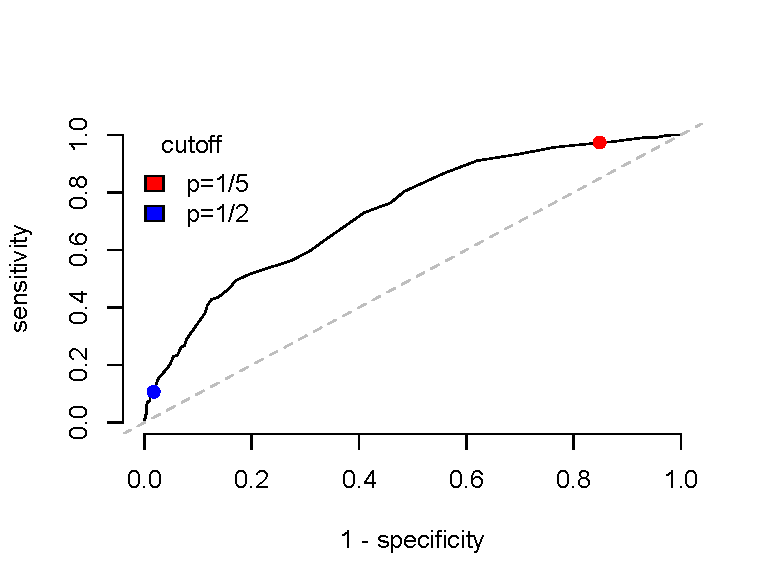
\includegraphics[width=4.25in]{CREDroc}


From signal processing: {\nv R}eceiver {\nv O}perating {\nv C}haracteristic.

A tight fit has the curve forced into the top-left corner.

\vskip -.5cm

\end{frame}

\begin{frame}
{Multinomial Logistic Regression}

Probabilities are the basis for good cost-benefit classification.

\vskip .1cm
We can get binary probabilities from binomial regression.

\vskip .5cm
In {\it multi-class} problems,  response $y$ is one of $K$ `categories'.

\vskip .1cm
Rewrite $\bm{y}_i = [0,1,\ldots,0]$, where $y_{ik}=1$ if response $i$ is class $k$.  

\vskip .5cm
Then we need a model for  
{\large\[\theme
\ds{E}[y_{ik} |\bm{x}_i] = f( \bm{x}_i'\bs{\beta}_k ).
\]}
$\Rightarrow$ we need a to fit regression coefficients $\bs{\beta}_k$ for {\it each} class.

\end{frame}

\begin{frame}
\vskip .1cm
To move to probabilites for multi-class problems, 
we need a Multinomial Regression for $\mr{p}(y_k = 1|\bm{x}) = p_k(\bm{x})$, $k=1\ldots K$.

\sk
Extend logistic regression via the {\theme multinomial logit}:
\[\nv
\mr{p}(y_j = 1|\bm{x}) = p_j(\bm{x}) = \frac{e^{\bm{x}'\bs{\beta_j}}}{
\sum_{k=1}^K e^{\bm{x}'{\bs{\beta_k}}}}
\]
{\theme Note separate coefficients for each class: 
$\bs{\beta}_{k}$.}

\vskip .1cm
Fitting this is called `multinomial logistic regression'.

\end{frame}

\begin{frame}
{Multinomial Logistic Regression}

Multinomial response is $y_{ik}$ for $k\in 1\ldots K$: a {\it class id}.

\vskip .1cm
Say $k_i$ is the class for observation $i$, so $y_{k_i}=1$.

\vskip .5cm
Given class probabilities $\bm{p}_i = [p_{i1} \ldots p_{iK}]$, we get
\[
\mr{LHD} \propto \prod p_{ik_i}  ~~~\text{and}~~~ \mr{Dev} \propto -2\sum_i \log(p_{ik_i})
\]
%\vskip -.25cm{\gr
% where each probability is $p_{iy_i} = 
% \exp[\alpha_{y_i} +\bm{x}_i\beta_{y_i}]/\sum_{k=1}^K e^{\alpha_k + \bm{x}_i{\bs{\beta_k}}}$,
% so the deviance is $\propto \sum_i\log\left(\sum_{k=1}^K e^{\alpha_k + \bm{x}_i{\bs{\beta_k}}}\right) - [\alpha_{y_i} +\bm{x}_i\beta_{y_i}]$}.


We'll fit these the usual way: penalized deviance minimization.
\[
\mr{min} \left\{ -\frac{2}{n}\sum_i \log p_{ik_i}(\bs{\beta}) + \sum_k \sum_j\lambda |\beta_{kj}|\right\}
\]
You can also have $\lambda_k$: different penalty for each class.

\end{frame}

\begin{frame}

Fit the model in {\tt glmnet} with {\tt family="multinomial".}

\vskip .25cm
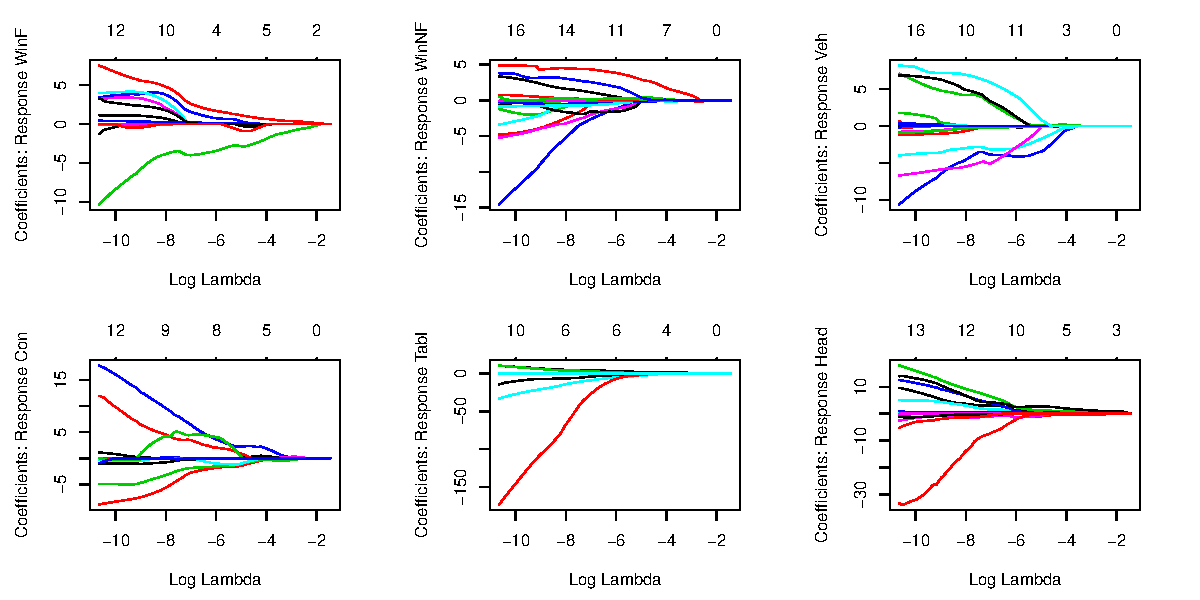
\includegraphics[width=4.25in]{../graphs/fglPATHS}

\vskip .25cm
A separate path plot for every class.  \\\gr See {\tt glass.R}  for
coefficients, prediction, and other details.
\end{frame}

\begin{frame}

We can do OOS experiments on {\it multinomial deviance}.

\vskip .25cm
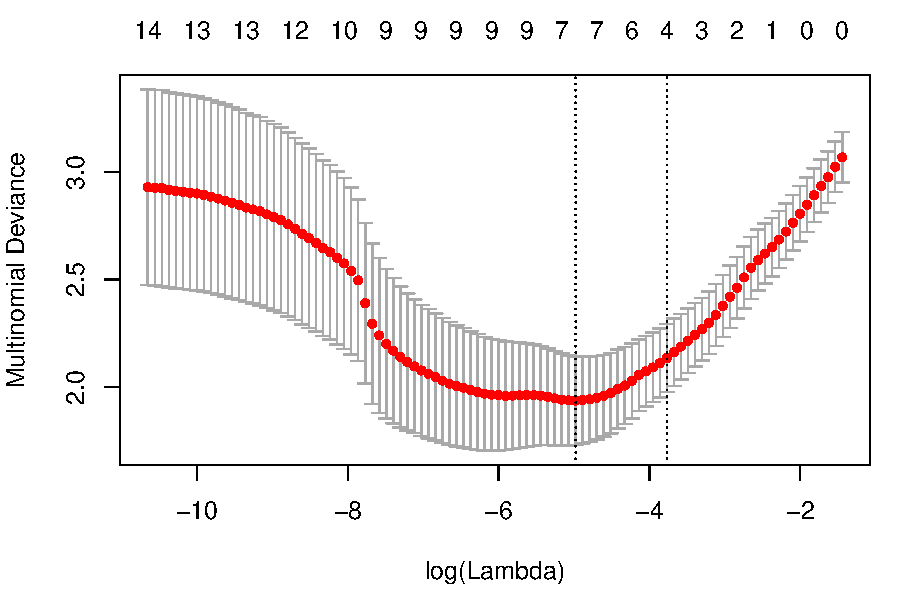
\includegraphics[width=4.25in]{../graphs/fglCV}

And use this to choose $\lambda$ (one shared for all classes here).
\vskip -.25cm

\end{frame}

\begin{frame}

The `fit plot' for multinomials:  $\hat p_{i k_i}$, prob of true class, on $k_i$.

~~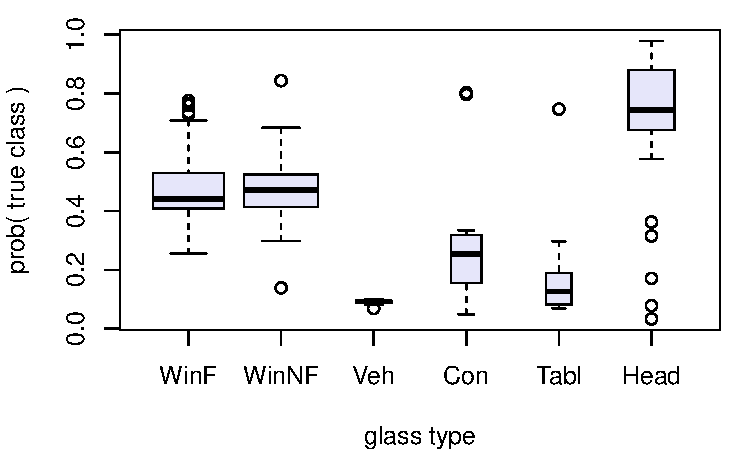
\includegraphics[width=4in]{../graphs/fglFIT}

\vskip .25cm
{\gr {\tt Veh}, {\tt Con}, {\tt Tabls} have low fitted probabilities, but they are generally more rare in this sample (width of box is $\propto$ count).}
\end{frame}

\begin{frame}
{MN classification via decision costs}

{Suppose a simple cost matrix has}
\begin{center}
\begin{tabular}{r|cccccc}
&{\tt WinF} & {\tt WinNF} & {\tt Veh} & {\tt Con} & {\tt Tabl} & {\tt Head}\\
\cline{2-7}
{$\hat k =${\tt Head}} & 9 & 9 & 9 & 9 & 9 & 0\\
{$\hat k \neq ${\tt Head} } & 0 & 0 & 0 & 0 & 0 &1 \\
\end{tabular}
\end{center}
e.g. a court case where {\tt Head} is evidence for the prosecution\\
{\gr (innocent until proven guilty, and such).}

\vskip .25cm
Then expected cost of $\hat k \neq {\tt Head}$ is greater than $\hat k = {\tt Head}$ if
\[
p_{\tt head} > 9(1-p_{\tt head})  ~~\Leftrightarrow~~ p_{\tt head} > 0.9
\] 


\vskip .25cm If you don't have asymmetric costs, \\ just use a {\nv maximum probability rule}: $\nv \hat k = \mr{argmax}_k ~\hat p_k$.

You can get this in R with {\tt apply(probs,1,which.max)}.

\end{frame} 

\begin{frame}[fragile]
{Interpreting the MN logit}


{We're estimating a function that sums to one across classes.\\
But now there are $\nv K$ categories, instead of just two.}

\vskip .25cm
The log-odds interpretation now compares between classes: 
{\nv
\[
\log\left(\frac{p_a}{p_b}\right) = 
\log\left(\frac{e^{\bm{x}'\bs{\beta}_a}}{e^{\bm{x}'\bs{\beta}_b}}\right) =
\bm{x}[ \bs{\beta}_a-\bs{\beta}_b].
\]}
For example, with a one unit increase in {\tt Mg}:
\begin{semiverbatim}\gr\small
# odds of non-float over float drop by 30-40\%\nv 
exp(B["Mg","WinNF"]-B["Mg","WinF"]) \bk
 0.6633846\gr
# odds of non-float over Con increase by 60-70\%\nv
exp(B["Mg","WinNF"]-B["Mg","Con"]) \bk
 1.675311
\end{semiverbatim}
\vskip -.5cm

\end{frame}

\begin{frame}[fragile]
{Interpreting the MN logit}


{Interactions also translate directly.
\\You just need to look at differences across class coefficients:}

\vskip .1cm
{\nv In my run, the {\tt RI:Mg} interaction coefficient is estimated as \\$\beta_{\tt winNF,RI:Mg} = -.05$ for {\tt WinNF} and 0 for both {\tt WinF} and {\tt Con}. 

\vskip .1cm  So the above odds {\it decrease} by 5\%  under every extra unit {\tt RI}.}

{\gr ($\exp(-0.05) \approx 0.95$; see code for more detail)}

\sk
$k$-against-others odds  are not as simple: 

\vskip .1cm
~~~~~~~~~~~log[$p_k/(1-p_k)$] = $\bm{x}\bs{\beta}_k 
- \log \sum_{j\neq k} e^{\bm{x}\bs{\beta}_j}$.
\vskip .2cm \hfill  A nonlinear function of $\bm{x}$!~~~~~~~~~~~~~~~~~

\vskip .2cm
All we can say is something like 

\vskip .1cm
\hfill {\it  Unit increase in $x_j$ multiplies odds numerator for class $k$  by $\beta_{kj}$. }
\end{frame}


\begin{frame}
{An alternative version of MN logit}

You might have noticed: multinomial regression can be slow...

\vskip .1cm
This is because everything needs to be done $K$ times!

\vskip .1cm
And each $\bs{\hat\beta}_k$ depends on the others:
$p_{ik} = e^{\bm{x}'\bs{\beta}_k}\theme/\sum_je^{\bm{x}'\bs{\beta}_j}$.


\vskip .5cm
It turns out that multinomial logistic regression is {\it very similar} to 
\[
\ds{E}[y_{ik} |\bm{x}_i] = \exp( \bm{x}_i'\bs{\beta}_k).
\]
That is, $K$ {\it independent} log regressions for each class $k$.


\vskip .5cm
{\gr The full regression is $y_{ik} \sim \mr{Poisson}( \exp[
\bm{x}_i'\bs{\beta}_k] )$, which is the glm for `count
response'.  Deviance is $\propto
\sum_{i=1}^n \exp( \bm{x}_i'\bs{\beta}_k) - y_i(\bm{x}_i'\bs{\beta}_k)$. }

\end{frame}


\begin{frame}
{Distributed Multinomial Regression}

Since each $y_{ik} \sim \mr{Poisson}( e^{\bm{x}_i'\bs{\beta}_k} )$ regression is independent, wouldn't it be faster to do these all at the same time? {\theme Yes!}


\vskip .5cm
{\tt dmr} function in the {\tt distrom} library does just this. 

In particular, {\tt dmr} minimizes
\[
\sum_{i=1}^n \exp( \bm{x}_i'\bs{\beta}_k) - y_i(\bm{x}_i'\bs{\beta}_k)
+ \lambda_k \sum_j |\beta_{jk}|
\]
along a path of $\lambda_k$ {\it in parallel for every response class $k$}.

We then use AICc to get a different $\hat\lambda_k$ for each $k$.

\vskip .5cm
You can use $\bs{\hat\beta}_1 \ldots \bs{\hat\beta}_K$ as if they are for a multinomial logit.  \\{\gr The intercepts differ from {\tt glmnet}'s, but that's a wash anyways.}

\end{frame}

\begin{frame}
{DMR}

 {\tt dmr} is a faster way to fit multinomial logit in parallel.  

 It's based on {\tt gamlr}, so the syntax will be familiar.

\vskip .5cm
{\tt dmr(cl, covars, counts, ...) }
\begin{itemize}
\item {\tt covars} is $\bm{x}$.
\item {\tt counts} is $\bm{y}$.  {\gr Can be a factor variable.}
\item {\tt ...} are arguments to {\tt gamlr}.
\item {\tt cl} is {\theme a parallel socket cluster}.
\end{itemize}
It takes {\tt coef} and {\tt predict} as you're used to.

\vskip .5cm
The returned {\tt dmr} object is actually a  list of $K$ gamlr objects, and you can call plot, etc, on each of these too if you want.


\end{frame}


\begin{frame}

{\bf`` {\theme to compute in parallel} ''}
\\ ~do many calculations at the same time on different processors.

\sk
Supercomputers have long used parallelism for massive speed.

Since 2000's, it has become standard to have many processor `cores' on consumer machines.  Even my phone has 4.

\sk  You can take advantage of this without even knowing.

\vskip .2cm
\begin{itemize}
\item Your OS runs applications on different cores.
\item Videos run on processing units with 1000s of tiny cores.
\end{itemize}

\vskip .2cm
And numeric software can be set up to use multiple processors.

{\gr e.g., if you build R `from source', you can set this up.}

\end{frame}

\begin{frame}[fragile]
{Parallel Computing in R}

{R's {\tt \nv parallel} library lets you take advantage of many cores.}

\vskip .1cm
It works by organizing {\it clusters} of processors.

\vskip .25cm
To get a cluster of cores do {\tt \theme  cl <- makeCluster(4)}

You can do {\tt detectCores()} to see how many you have.

{\gr If you're on a unix machine (mac/linux), you can ask for {\tt makeCluster(4,type="FORK")} and it will often be faster.}

\sk
After building {\tt cl}, just pass it  to {\tt dmr} and you're off to the [parallel] races.  Use {\tt stopCluster(cl)} when you're done.

\vskip .25cm\gr
Note: this requires your computer is setup for parallelization.  This {\it should} be true, but if not you can run {\tt dmr} with {\tt cl=NULL}.

\end{frame}

\begin{frame}
{DMR for glass data}

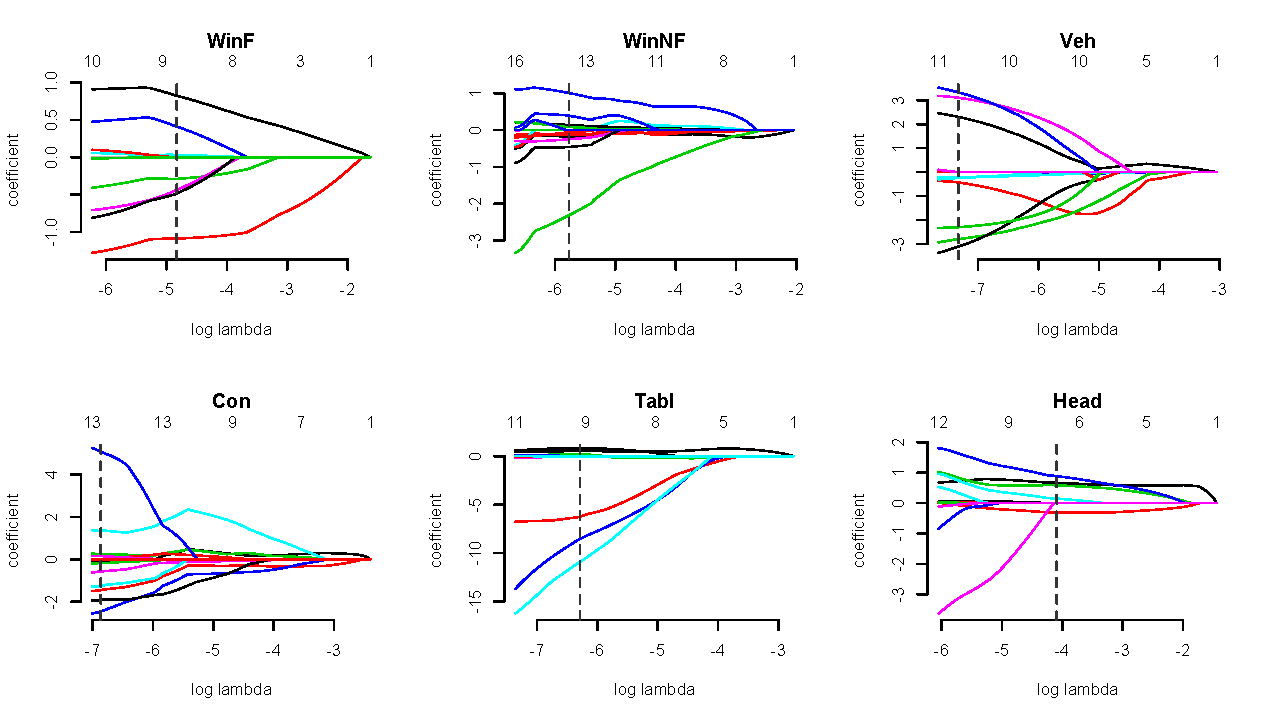
\includegraphics[width=4.25in]{fglDMR}

\vskip .25cm
The vertical lines show AICc selection: note it moves!

{\gr Note that {\tt glmnet} {\tt cv.min} rule chose $\log \hat\lambda \approx 5$.}

\end{frame}

\begin{frame}
{Massive Text Regressions}

The motivation for DMR actually comes from  text mining.

\vskip .5cm
The task is the estimate $\bs{\hat\beta}_k$ for $\ds{E}[y_{ik} |\bm{x}_i] = \exp( \bm{x}_i'\bs{\beta}_k)$\\ ~~~~~~~~ where $y_{ik}$ is the {\nv count for word $k$ in document $i$} \\ ~~~~~~~~~~~ and $\bm{x}_i$ are document attributes (author, date, etc).

\vskip .5cm
Sounds simple: just regression for word counts.

\vskip .1cm  However, you'll need to do this quickly for 100k-1mil words!  \\And the corpus of documents is far to big to fit on one computer.
\end{frame}


\begin{frame}

\begin{adjustwidth}{-.5in}{}
\vskip -.6in
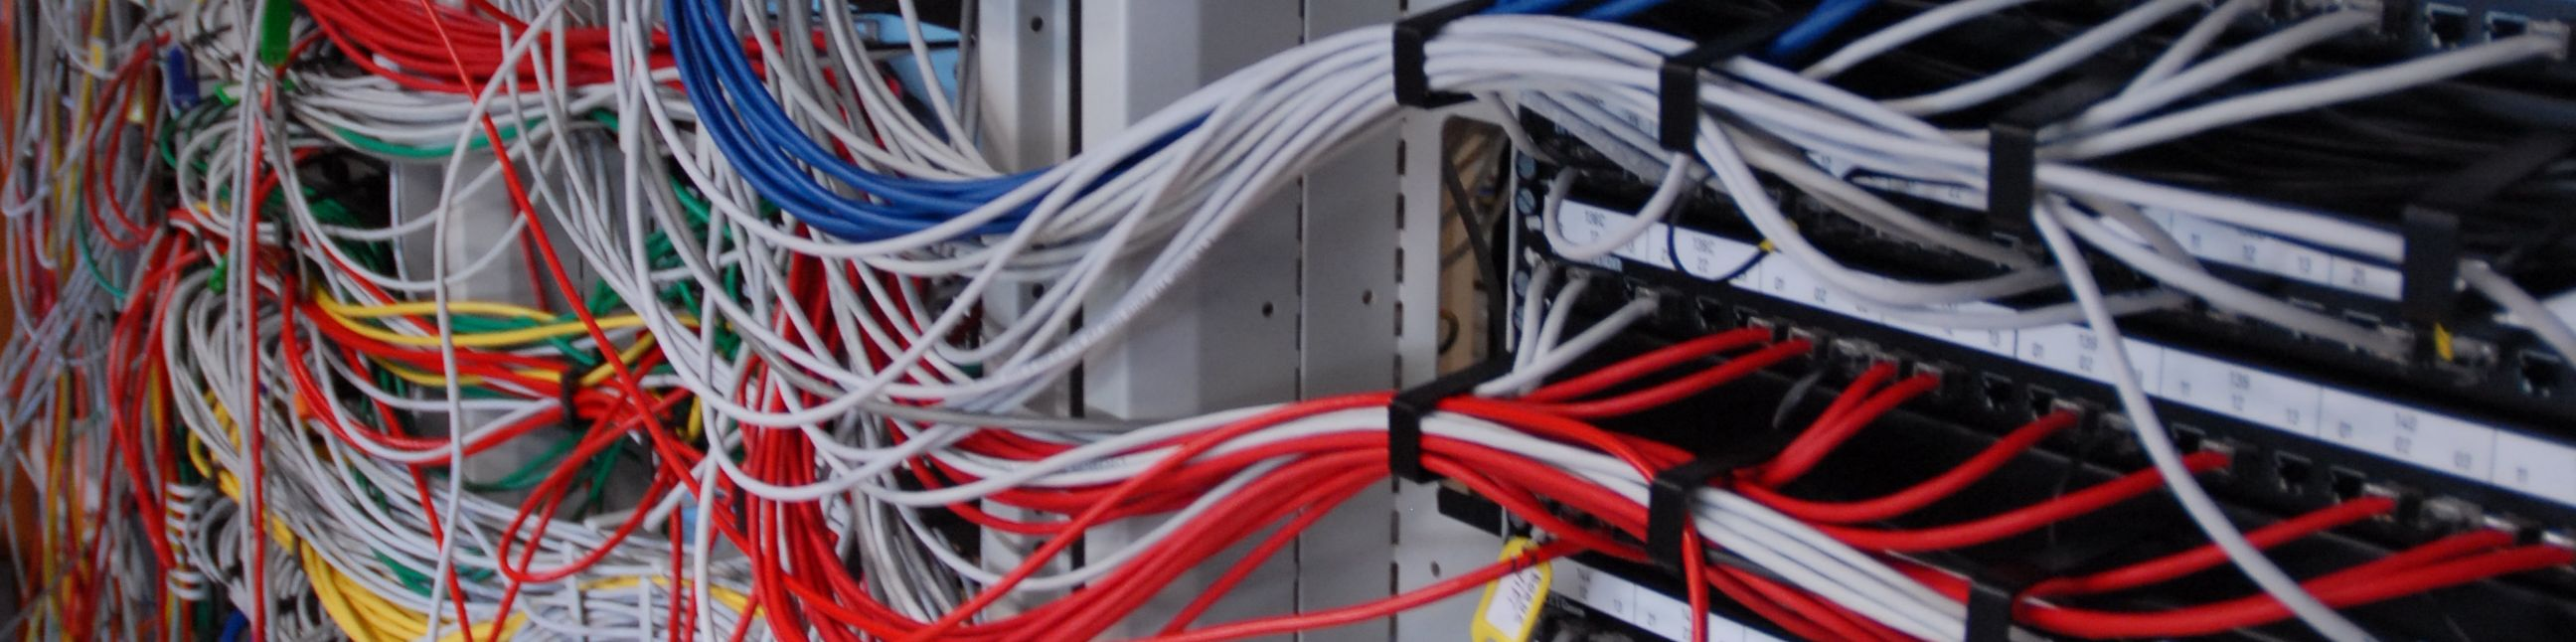
\includegraphics[width=6in]{../graphs/broadband}
\end{adjustwidth}

\vskip .6cm

{ \Large {\gr Diversion:} Data Distribution and Big Data}

\sk
{\nv Parallel}: many computations at once, using the same data.\\
{\nv Distributed}: independent computations on many datasets.\\

\sk
Parallel computing is good for large computations, \\but
for truly {\nv Big Data} we need distributed algorithms.

\sk
The DMR idea is distributable.

\end{frame}


\begin{frame}
{Take advantage of massive bandwidth}

\vskip .25cm
Storage systems like Hadoop's HDFS and Amazon's S3 split your  data into little
pieces {\gr (e.g. 64kb of a file)} that are kept wherever is convenient {\gr
(often in more than one place)}.

{\nv You interact only with a map of where things are.}

\vskip .25cm
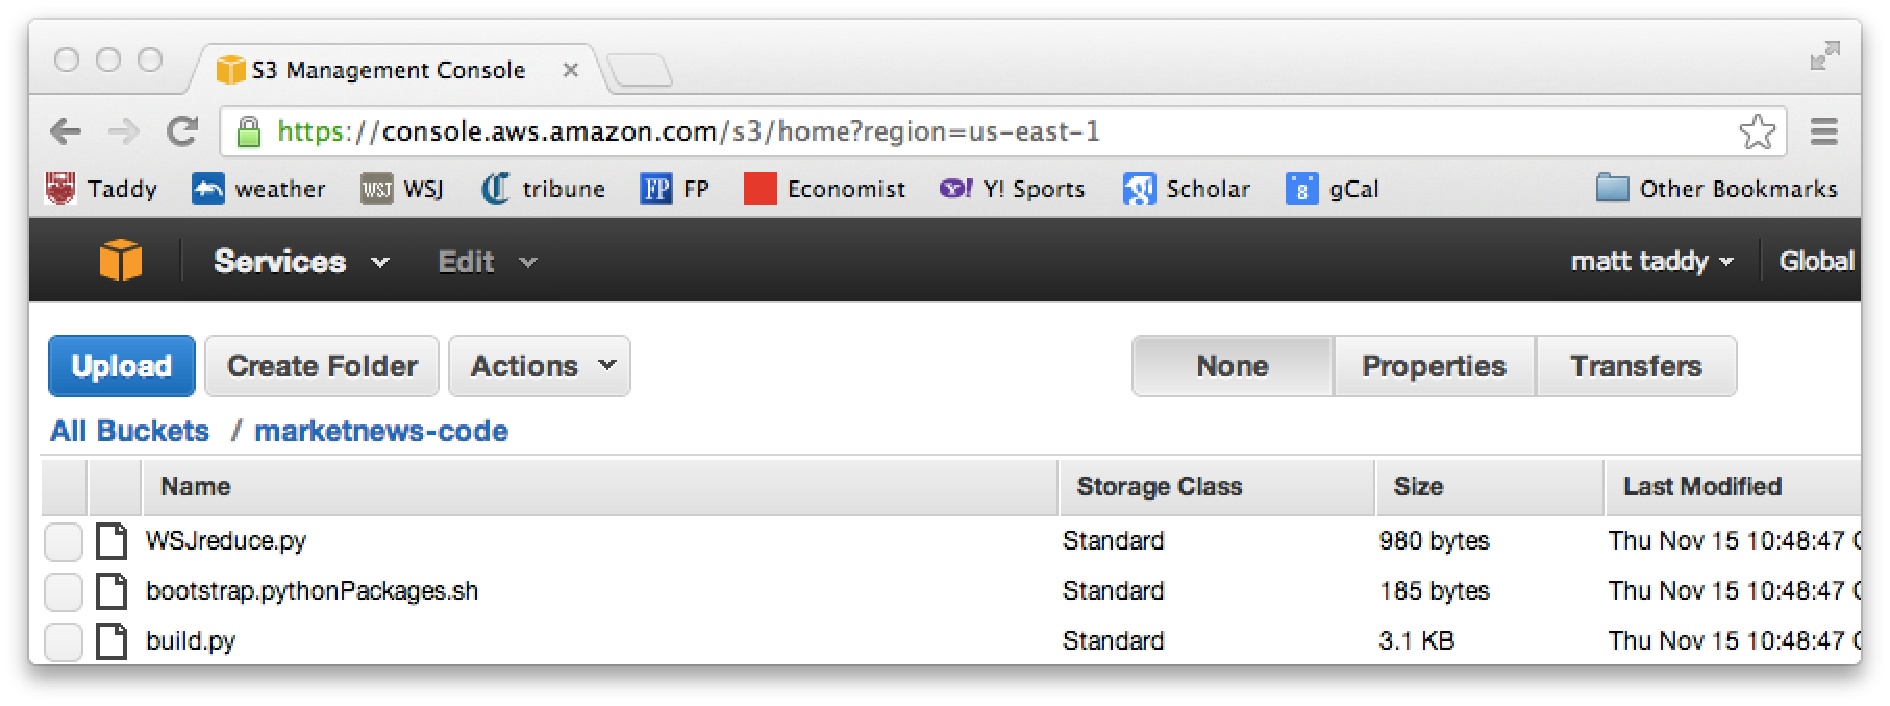
\includegraphics[width=4.25in]{../graphs/S3console}

\vskip .3cm
Much of database theory is gone.  \\
Just append new info and toss it in the cloud.\\

\vskip -.25cm
\end{frame}

\begin{frame}[fragile]
{Distributed Analysis with \theme MapReduce}

{Simple but  powerful {\nv algorithm framework: \it a recipe for
recipes}. } 

{\gr Publicized by Google around 2004, but ideas pre-date that.}

\sk
A Map-Reduce algorithm has three steps\\
{~~~\nv Map:} calculate and sort relevant statistics by key.\\
{~~~\gr Partition:} make sure records with the same key end up \\~~~~~~~~~~~~~~~~~~~on the same machine (this is the hadoop magic).\\
{~~~\nv Reduce:} apply some action by key.

\vskip .25cm Shared-key subsets are sorted
and dispatched to  `{\theme reducers}', each of which does some
statistical analysis of the data.

\sk
Easy: \nv
Streaming Hadoop with S3 storage on Amazon EMR.

\vspace{-.25cm}
{\footnotesize \sg
\begin{verbatim}
     EMR -input s3://indir -output s3://outdir
         -mapper s3://map.py -reducer s3://reduce.R
\end{verbatim}
}

\vskip -1cm
\end{frame}

\begin{frame}[fragile]


\includegraphics[width=1.25in]{../graphs/spark}

\vskip .2cm
MapReduce is great, but it is a pretty rigid recipe.  

\vskip .2cm
Many models are fit by {\it iteration}: update the model, look at what happened, then make another set of updates.

\vskip .2cm
One can chain together MapReduce steps.  But MR writes to disk after each run, so this will include tons of I/O slowness.

\vskip .2cm
Instead: Spark!  It is just like MR, except that the results and data stay `in memory' on each machine until you are done.  

\vskip .2cm
Spark is getting closer to mainstream.  \\Runs on EMR, but you need to write in python or scala.  \\ sparkR exists, but you need your own cluster...  

\end{frame}

\begin{frame}
{Back to big text regressions}

Consider raw documents stored in a distributed file system \\(i.e., many different machines) such as HDFS or Amazon S3.

\vskip .5cm
{\nv A MapReduce Algorithm}

\vskip .1cm Map: parse documents to output lines {\tt word  docid|count}.

\vskip .1cm Partition: All lines for given word $k$ go to same machine.

\vskip .1cm Reduce: regress counts for $k$ onto the doc attributes, \\~~~~~~~select optimal $\hat{\bs{\beta}}_k$ and send just this back to head.

\vskip .1cm
{\nv Collect all $\hat{\bs{\beta}}_1\ldots\hat{\bs{\beta}}_K$ and you've got your text model!}

\vskip .5cm 
Massively scalable: build out not up.

\gr
Distributed computing is something we can discuss if you want with your project.  The tools are open source and require tech savvy. You'll want to be solid on fundamentals before diving in.

\end{frame}


\end{document}
